% Point d'avancement tuteur, 7 aout 2026. Compile avec Tectonic (pdfLaTeX standard).
% Perimetre : continuite directe du 31/07 (les 4 pistes du call Hugo). Ce point porte sur la
% ROBUSTESSE et la DEFENSE du modele : reponse a la remarque de Caroline Hillairet (le SCR est
% un quantile d'un objet incertain), les trois etages d'incertitude, validation, benchmark, ROI,
% et l'approfondissement de P4 (sous-process, temps d'arret).
\documentclass[11pt]{beamer}
\usetheme{Madrid}
\usecolortheme{seahorse}
\usepackage[utf8]{inputenc}
\usepackage[T1]{fontenc}
\usepackage[french]{babel}
\usepackage{booktabs}
\usepackage{amsmath,amssymb}
\usepackage{eurosym}
\graphicspath{{../vasicek_lab/figures/}{../cascade_qualitative/figures/}}
\setbeamertemplate{navigation symbols}{}
\setbeamertemplate{caption}{\raggedright\insertcaption\par}
\setbeamerfont{block title}{size=\small}

\title[Point d'avancement]{Mémoire SCR DORA : point d'avancement}
\subtitle{Suites de la dernière réunion, et la remarque de Caroline Hillairet}
\author[K. Kaddouri]{Kélian Kaddouri}
\institute[ENSAE / Nexialog]{ENSAE / Nexialog Consulting}
\date[07/08/2026]{7 août 2026}

\begin{document}

\begin{frame}
\titlepage
\end{frame}

% =====================================================================
\begin{frame}{Depuis le dernier point}
La dernière réunion a traité les \textbf{quatre pistes} du call (loi de comptage NB, seuil de
déclenchement de P4, décomposition $W=S+A$ / martingale, KPI pilotables). Ce point les
\textbf{poursuit}, sans rajouter de brique : il fait passer le modèle de \textbf{construit} à
\textbf{défendable}, autour de deux fils.
\vfill
\begin{block}{Le fil de ce point}
\textbf{(1) La remarque de Caroline Hillairet} : le SCR est un quantile d'un objet incertain.
Elle conduit à \textbf{expliciter l'incertitude} et à \textbf{valider} le socle.\\[3pt]
\textbf{(2) La direction de la contagion}, que je n'arrivais pas à calibrer : elle se cherche
\textbf{ailleurs que dans les bases de données}, et j'ai besoin d'un service sur ce point.\\[3pt]
\textbf{(3) L'approfondissement de P4} : le sous-process tiers, puis le déclenchement comme
\textbf{temps d'arrêt}, qui referme le fil vers la martingale.
\end{block}
\end{frame}

% =====================================================================
\begin{frame}{La remarque de Caroline : un quantile d'un objet incertain}
\og{}Prendre le quantile de quelque chose d'incertain est mauvais.\fg{}
\medskip

Le SCR est une VaR $99{,}5\,\%$ : un point de la queue, lu là où les données sont les plus
rares. Sur nos données, son seul intervalle de confiance vaut déjà un \textbf{facteur 2,6}.
\vfill
\begin{block}{La réponse}
On ne peut pas abandonner la VaR (elle est \emph{imposée} par le cadre prudentiel). On
\textbf{explicite} donc l'incertitude, sur trois étages qui se cumulent : \textbf{paramètre}
(bootstrap sur $\xi$), \textbf{identification} (bornes sur la direction $W$), et \textbf{modèle}
(le choix de la famille elle-même). Loin d'attaquer l'approche, la remarque en est la
justification.
\end{block}
\end{frame}

% =====================================================================
\begin{frame}{Les trois étages de l'incertitude}
\begin{center}
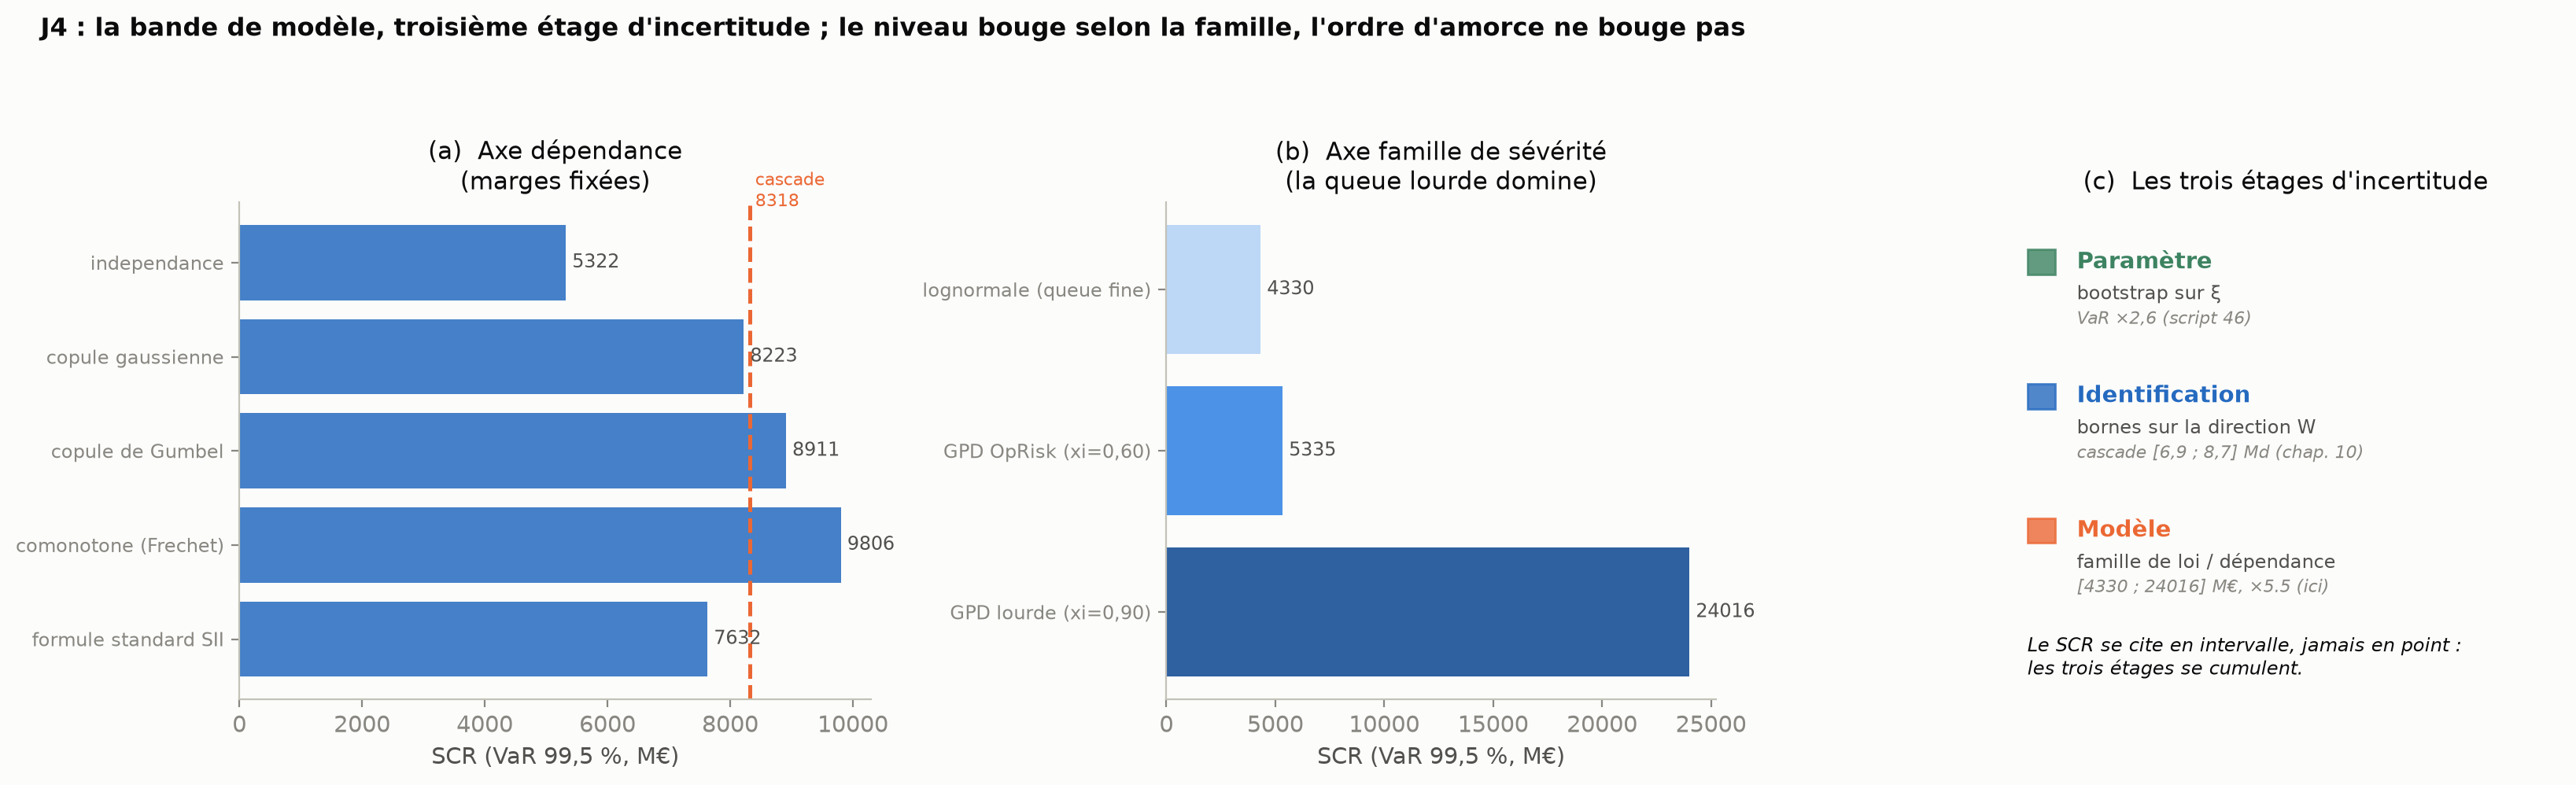
\includegraphics[width=\linewidth]{J4_bande_modele.png}
\end{center}
\vfill
\footnotesize À marges fixées, la structure de \textbf{dépendance} déplace le SCR d'un facteur
$1{,}8$ (indépendance à comonotone), notre cascade tombant entre les copules gaussienne et de
Gumbel ; la \textbf{famille de queue}, d'un facteur $5{,}5$. \textbf{Le niveau bouge dans la
bande, l'ordre des piliers ne bouge pas} --- c'est la thèse du mémoire, chiffrée sur un
troisième axe.
\end{frame}

% =====================================================================
\begin{frame}{Deux façons honnêtes de reporter le SCR}
\begin{columns}
\begin{column}{0.5\linewidth}
\centering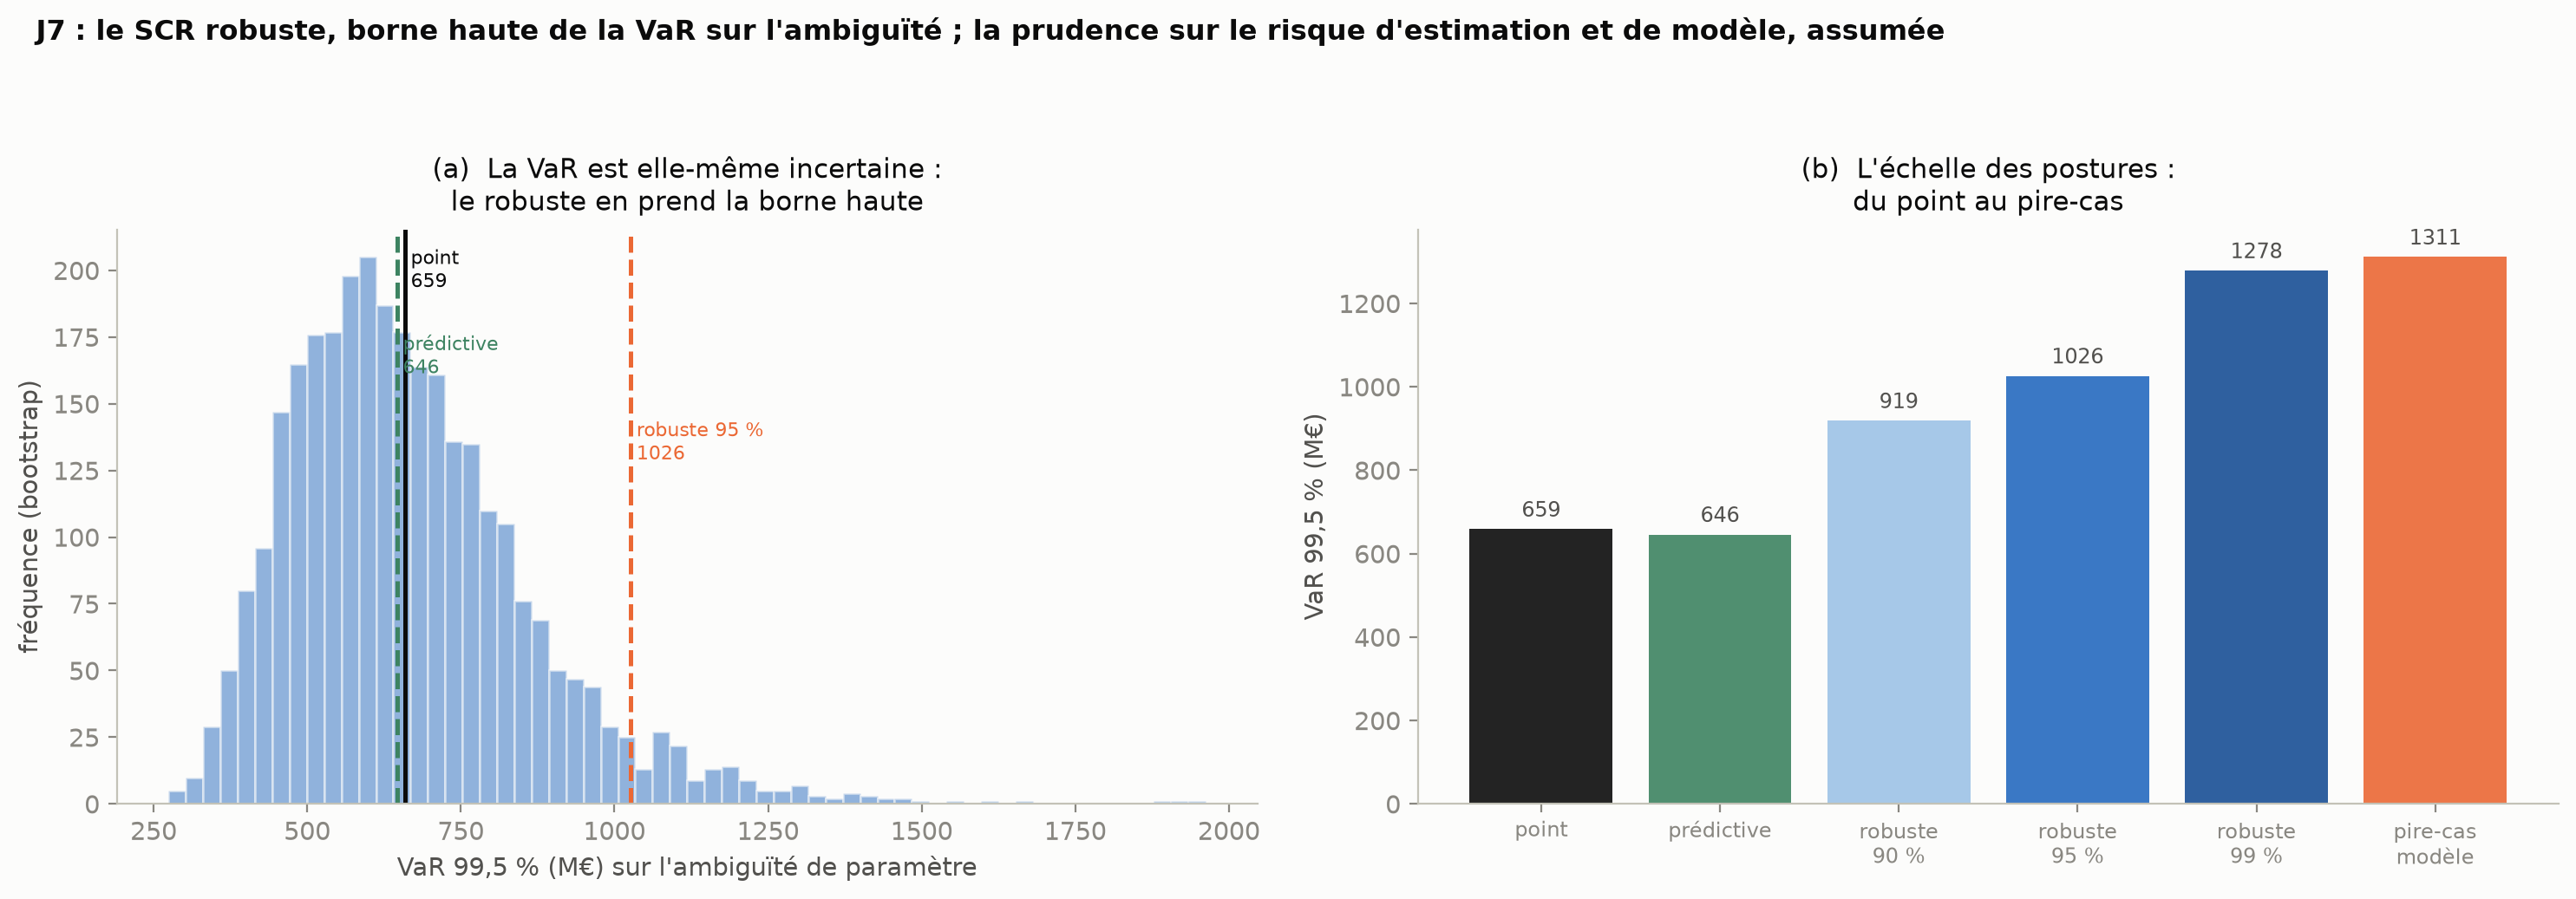
\includegraphics[width=\linewidth]{J7_scr_robuste.png}
\end{column}
\begin{column}{0.48\linewidth}
\small
\textbf{VaR prédictive} : on intègre l'incertitude \emph{avant} de prendre le quantile
(mélange sur le bootstrap). Résultat : à $99{,}5\,\%$ elle est \emph{quasi égale} au point.
La fragilité est dans la \textbf{largeur} de la bande, pas dans le point.
\medskip

\textbf{VaR robuste} : la \textbf{borne haute} sur l'ensemble d'ambiguïté. La robuste à
$95\,\%$ vaut $1{,}6\times$ le point ; le pire-cas de modèle, davantage encore.
\end{column}
\end{columns}
\vfill
\begin{block}{}
Deux points \emph{honnêtes} (prédictif, prudent) plutôt qu'un point \emph{trompeur}
(\emph{plug-in} nu). Le choix relève de la politique prudentielle. C'est la justification, et
non la remise en cause, de la thèse \og{}on lit le SCR en bande\fg.
\end{block}
\end{frame}

% =====================================================================
\begin{frame}{Le socle passe les tests d'adéquation}
\begin{center}
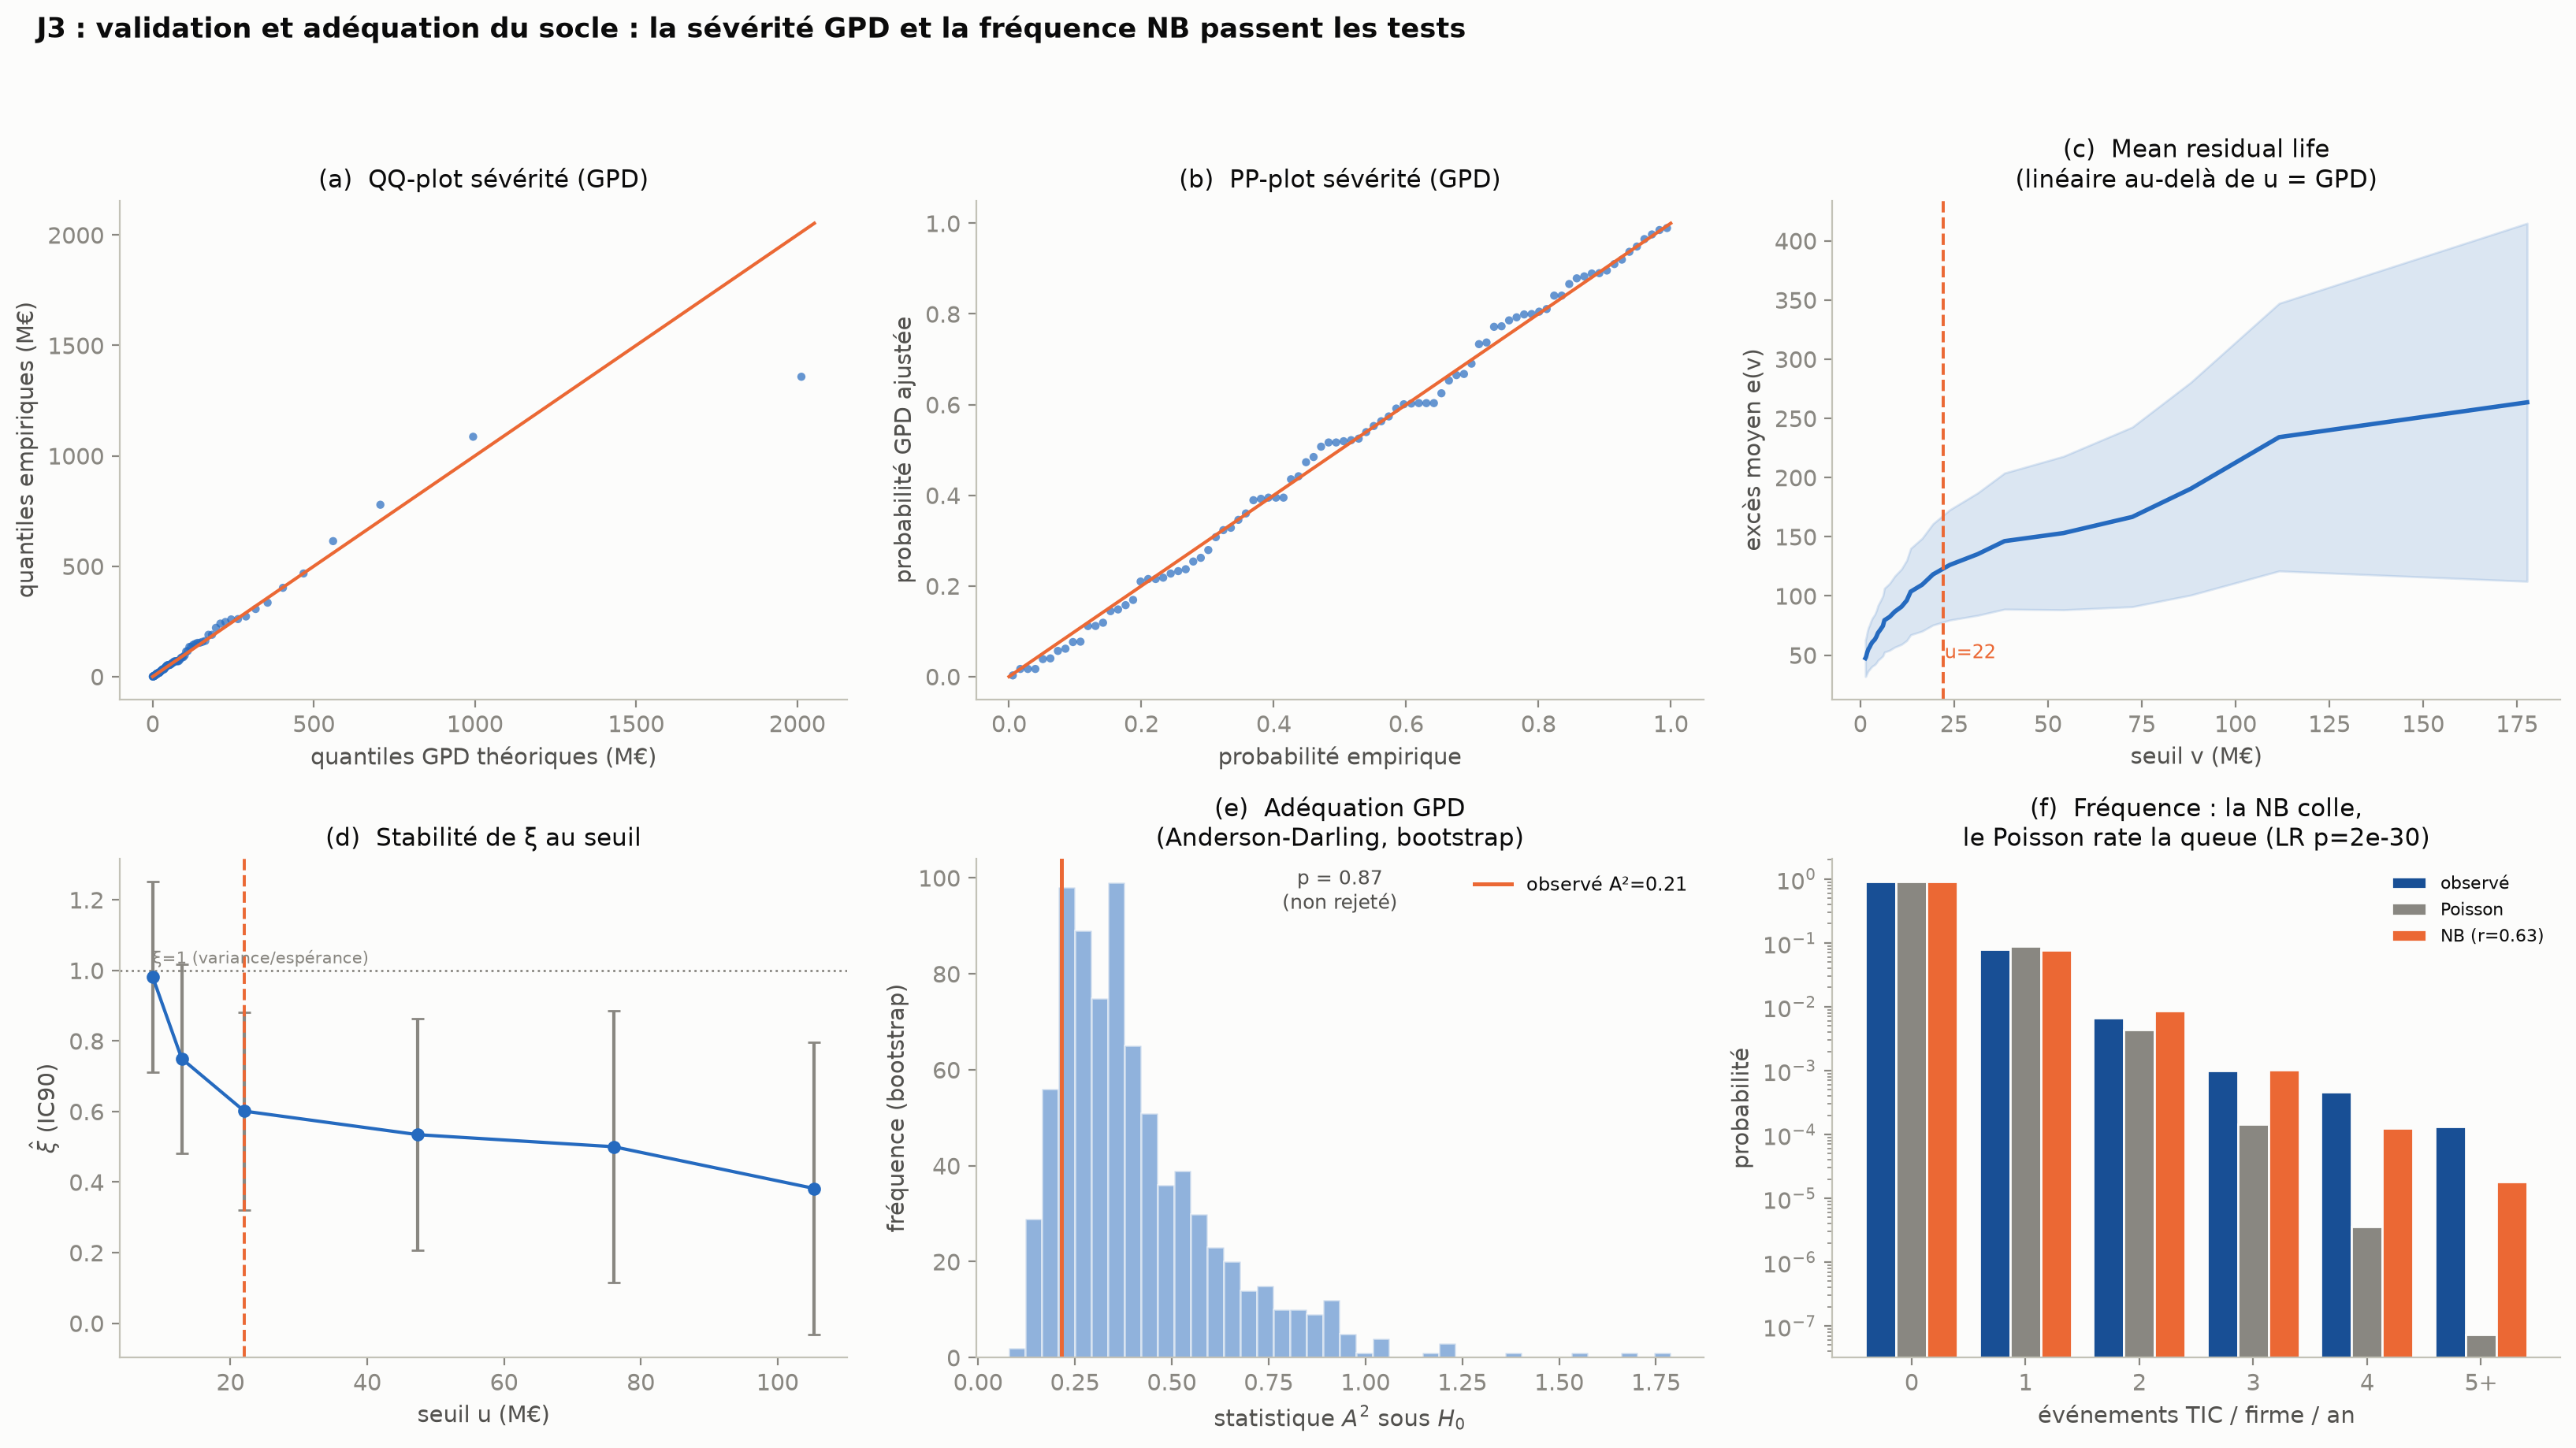
\includegraphics[width=\linewidth]{J3_validation_adequation.png}
\end{center}
\vspace{-1mm}
\footnotesize\centering Ce qu'un jury actuariel cherche en premier : les deux briques qui
portent le SCR s'ajustent-elles vraiment aux données ?
\end{frame}

% =====================================================================
\begin{frame}{Validation : ce que disent les tests}
\textbf{Sévérité GPD} --- elle passe sans réserve.
\begin{itemize}\itemsep2pt
\item QQ et PP-plots sur la diagonale ; vie résiduelle moyenne linéaire au-delà du seuil
      (signature GPD) ; $\hat\xi$ stable autour de $0{,}60$.
\item Tests non rejetés, $p$-value par \textbf{bootstrap paramétrique} (les valeurs tabulées ne
      valent pas quand les paramètres sont estimés) : Anderson-Darling $p=0{,}87$, KS $p=0{,}87$.
\item Couverture réelle de l'IC$_{90}$ de $\xi$ : $86\,\%$, proche du nominal.
\end{itemize}
\medskip
\textbf{Fréquence NB} --- sur $14\,944$ cellules firme-année, elle domine le Poisson sans
ambiguïté ($p\approx 10^{-30}$) ; la surdispersion est un fait.
\vfill
\begin{block}{}
Les tests portent sur la \textbf{forme} des lois, pas sur le \textbf{niveau} : la GPD et la NB
sont les bons objets, mais l'incertitude sur $\xi$ (donc sur la VaR) reste entière. Adéquation
n'est pas certitude --- d'où la lecture en bande.
\end{block}
\end{frame}

% =====================================================================
\begin{frame}{La direction, cherchée ailleurs que dans les bases}
\small
Aucune base publique ne mesure le \emph{sens} de la contagion, et le mémoire en fait un
résultat. Mais l'information existe ailleurs : après chaque grand incident, une \textbf{enquête
publique} reconstitue la séquence des défaillances. C'est la donnée qui manquait, à l'intérieur
d'un document et non d'une base.
\vfill
\begin{block}{Sept rapports dépouillés}
Microsoft Exchange, TSB, Equifax, Knight Capital, Capital One, ION, MOVEit.
\textbf{17 enchaînements} codés, protocole explicite.
\end{block}
\begin{block}{}
Le test placebo est cette fois \textbf{franchi} ($z=+3{,}9$ contre $-0{,}33$ sur les bases
agrégées), \textbf{aucun} enchaînement ne va à contre-sens, et la \textbf{gouvernance n'est
jamais une cible} quand la \textbf{gestion des incidents} est un aboutissement : la structure
du classeur, retrouvée par un chemin indépendant.
\end{block}
\end{frame}

% =====================================================================
\begin{frame}{Ce que cette information vaut, et laquelle chercher d'abord}
\begin{center}
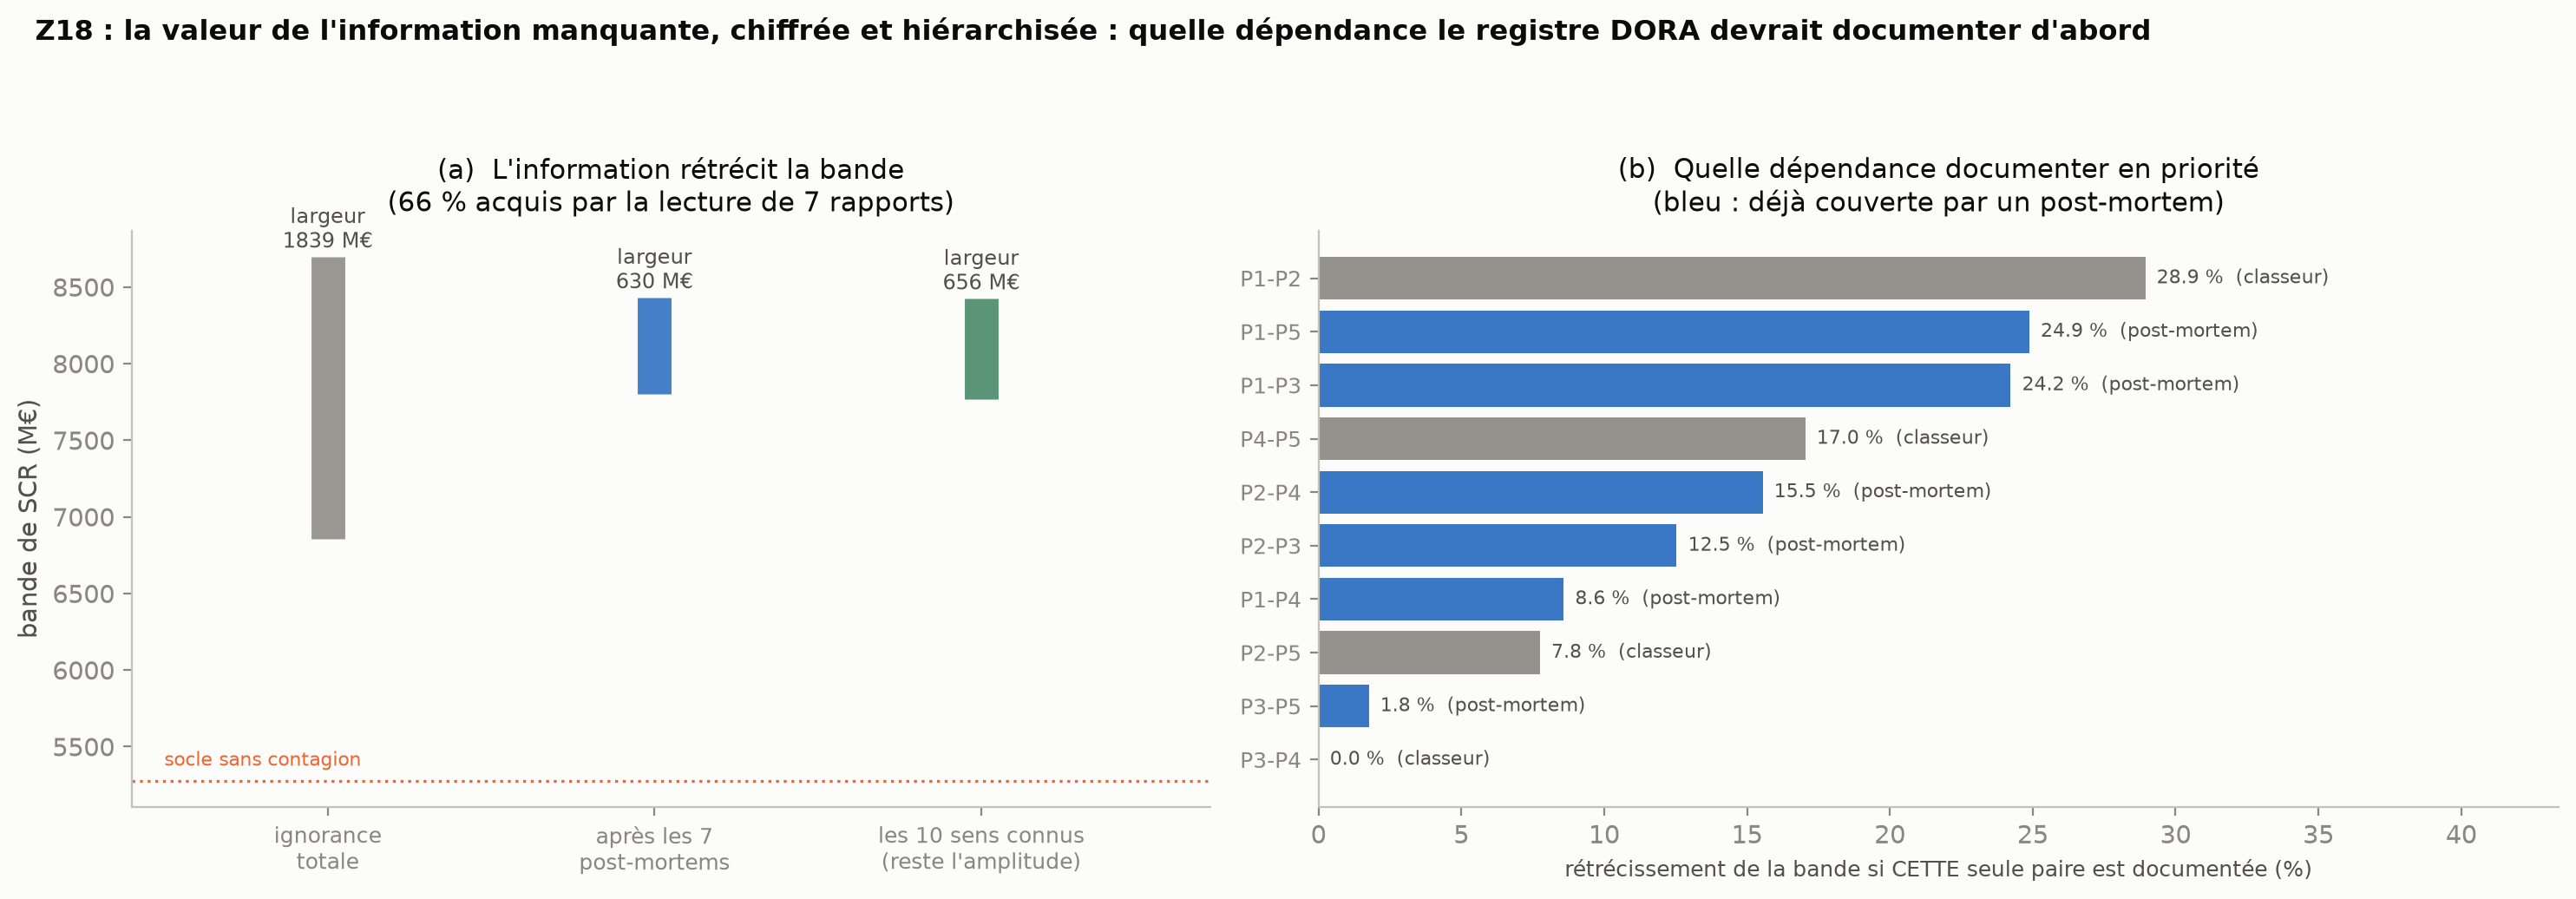
\includegraphics[width=\linewidth]{Z18_valeur_information.png}
\end{center}
\vspace{-2mm}
\small
Lire ces sept rapports a levé \textbf{66 \%} de l'ambiguïté sur la direction. Surtout, cette
valeur se \textbf{hiérarchise} : documenter une seule dépendance (gouvernance vers gestion des
incidents) en lèverait \textbf{29 \%} à elle seule, une autre n'en lèverait \emph{rien}. La
recommandation faite au régulateur cesse d'être générique. Et la dépendance la plus précieuse
est justement celle que les rapports ne couvrent pas.
\end{frame}

% =====================================================================
\begin{frame}{Ce que je ne revendique pas, et le service que je demande}
\begin{center}\small
\renewcommand{\arraystretch}{1.3}
\begin{tabular}{@{}l l l@{}}
\toprule
\textbf{Objet} & \textbf{Ce que j'ai} & \textbf{Posture} \\
\midrule
La structure d'ensemble & 17 enchaînements cohérents & \textbf{revendiquée} \\
Le sens de chaque lien & 2 paires sur 6 concluantes & \textbf{non revendiquée} \\
La force des liens & rien, et rien ne la donnera & \textbf{hors d'atteinte} \\
\bottomrule
\end{tabular}
\end{center}
\vfill
\begin{block}{La faiblesse que je préfère traiter plutôt que subir}
\small Ce dépouillement, \textbf{je l'ai fait seul}. Et une enquête officielle cherche un
responsable : elle conclut presque toujours à un défaut de gouvernance. L'ordre trouvé pourrait
donc refléter la \textbf{façon dont ces rapports sont écrits} plutôt que la réalité du terrain.
\end{block}
\begin{block}{D'où deux demandes, courtes et sans mathématiques}
\small Un \textbf{codage en aveugle} par quelqu'un qui ignore mes conclusions (45 min), et une
\textbf{relecture de praticien} (30 min). Dans les deux cas, un désaccord m'est plus utile
qu'un accord.
\end{block}
\end{frame}

% =====================================================================
\begin{frame}{P4 au niveau sous-process : ce qu'on ancre avant Mehdi}
\begin{center}
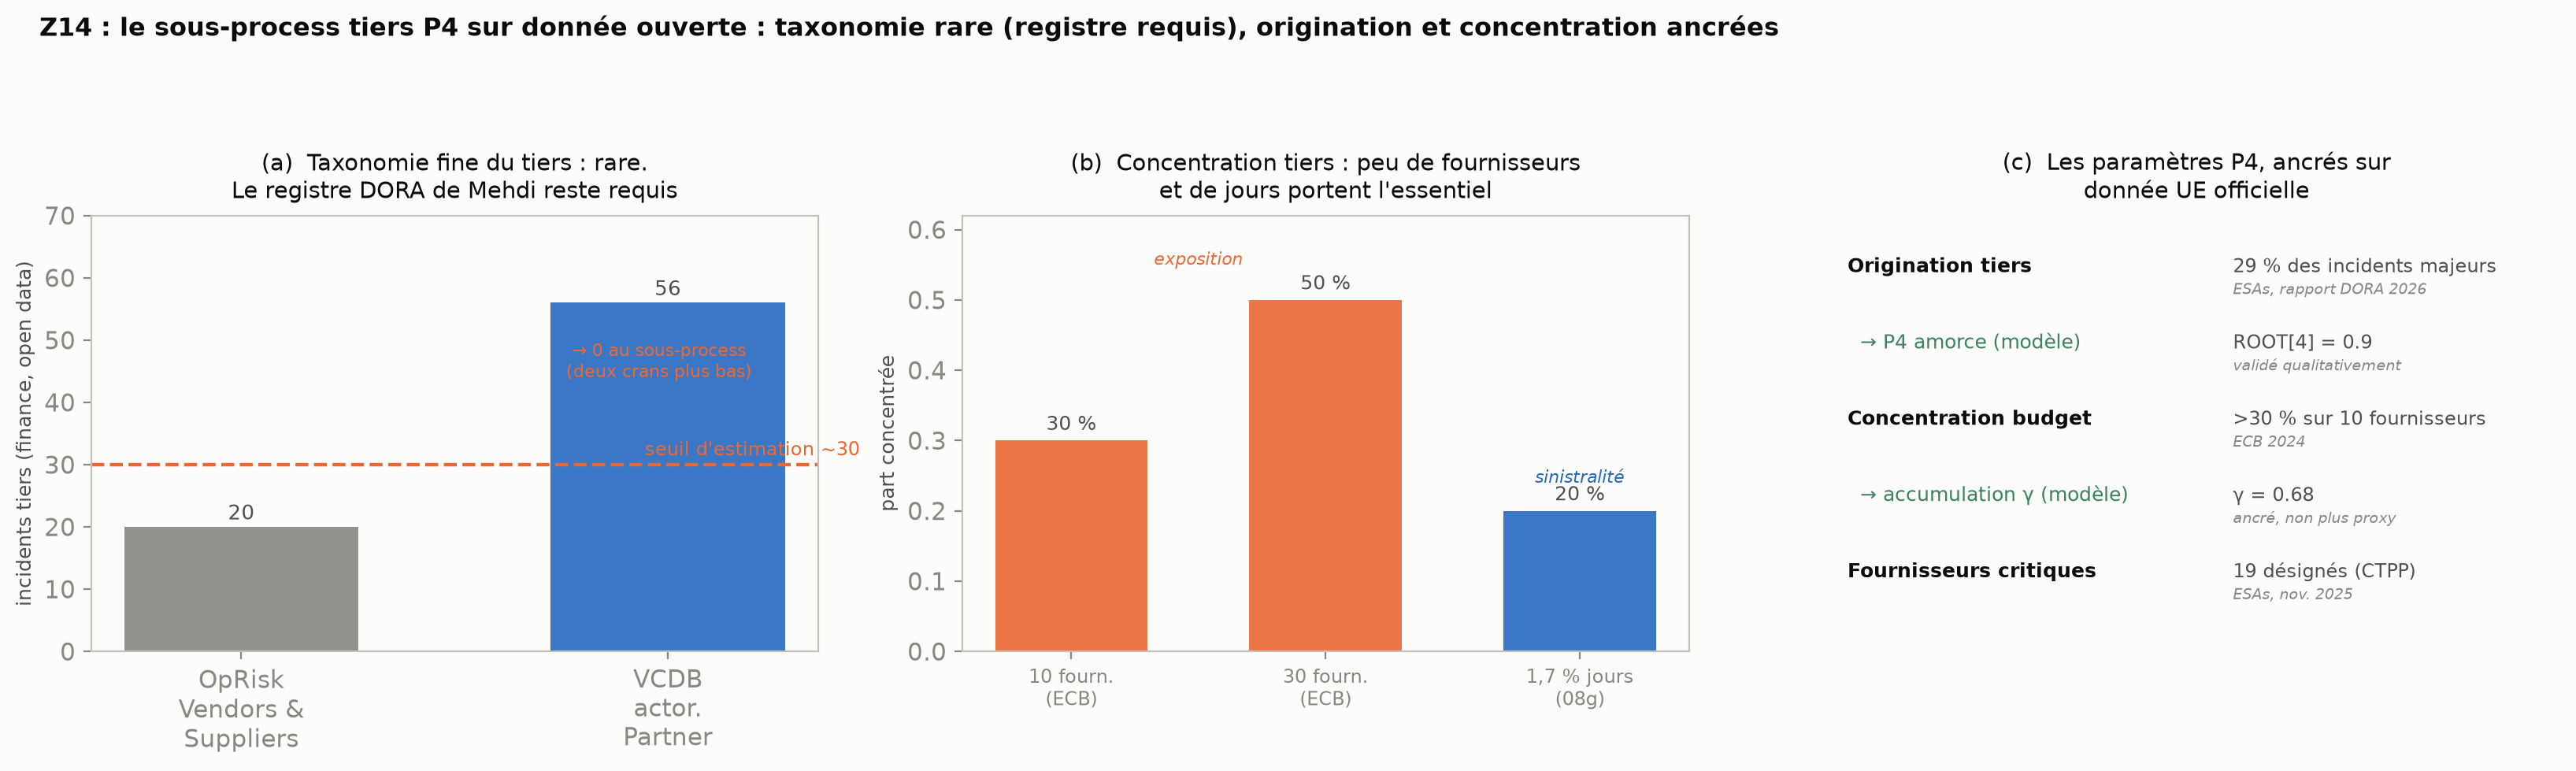
\includegraphics[width=\linewidth]{Z14_p4_sousprocess_open.png}
\end{center}
\vspace{-2mm}
\small
Deux constats opposés. La \textbf{taxonomie fine} du tiers est rare sur donnée ouverte (OpRisk
$20$, VCDB $56\!\to\!0$) : le registre DORA de Mehdi reste requis. Mais l'\textbf{origination}
($29\,\%$ des incidents majeurs d'origine tierce, ESAs 2026) et la \textbf{concentration} ($>$30~\%
du budget sur $10$ fournisseurs, BCE) sont ancrées sur donnée européenne officielle : elles
valident P4 comme amorce majeure et ancrent le paramètre d'accumulation $\gamma$.
\end{frame}

% =====================================================================
\begin{frame}{Le fil se referme : le déclenchement comme temps d'arrêt}
\begin{columns}
\begin{column}{0.55\linewidth}
\centering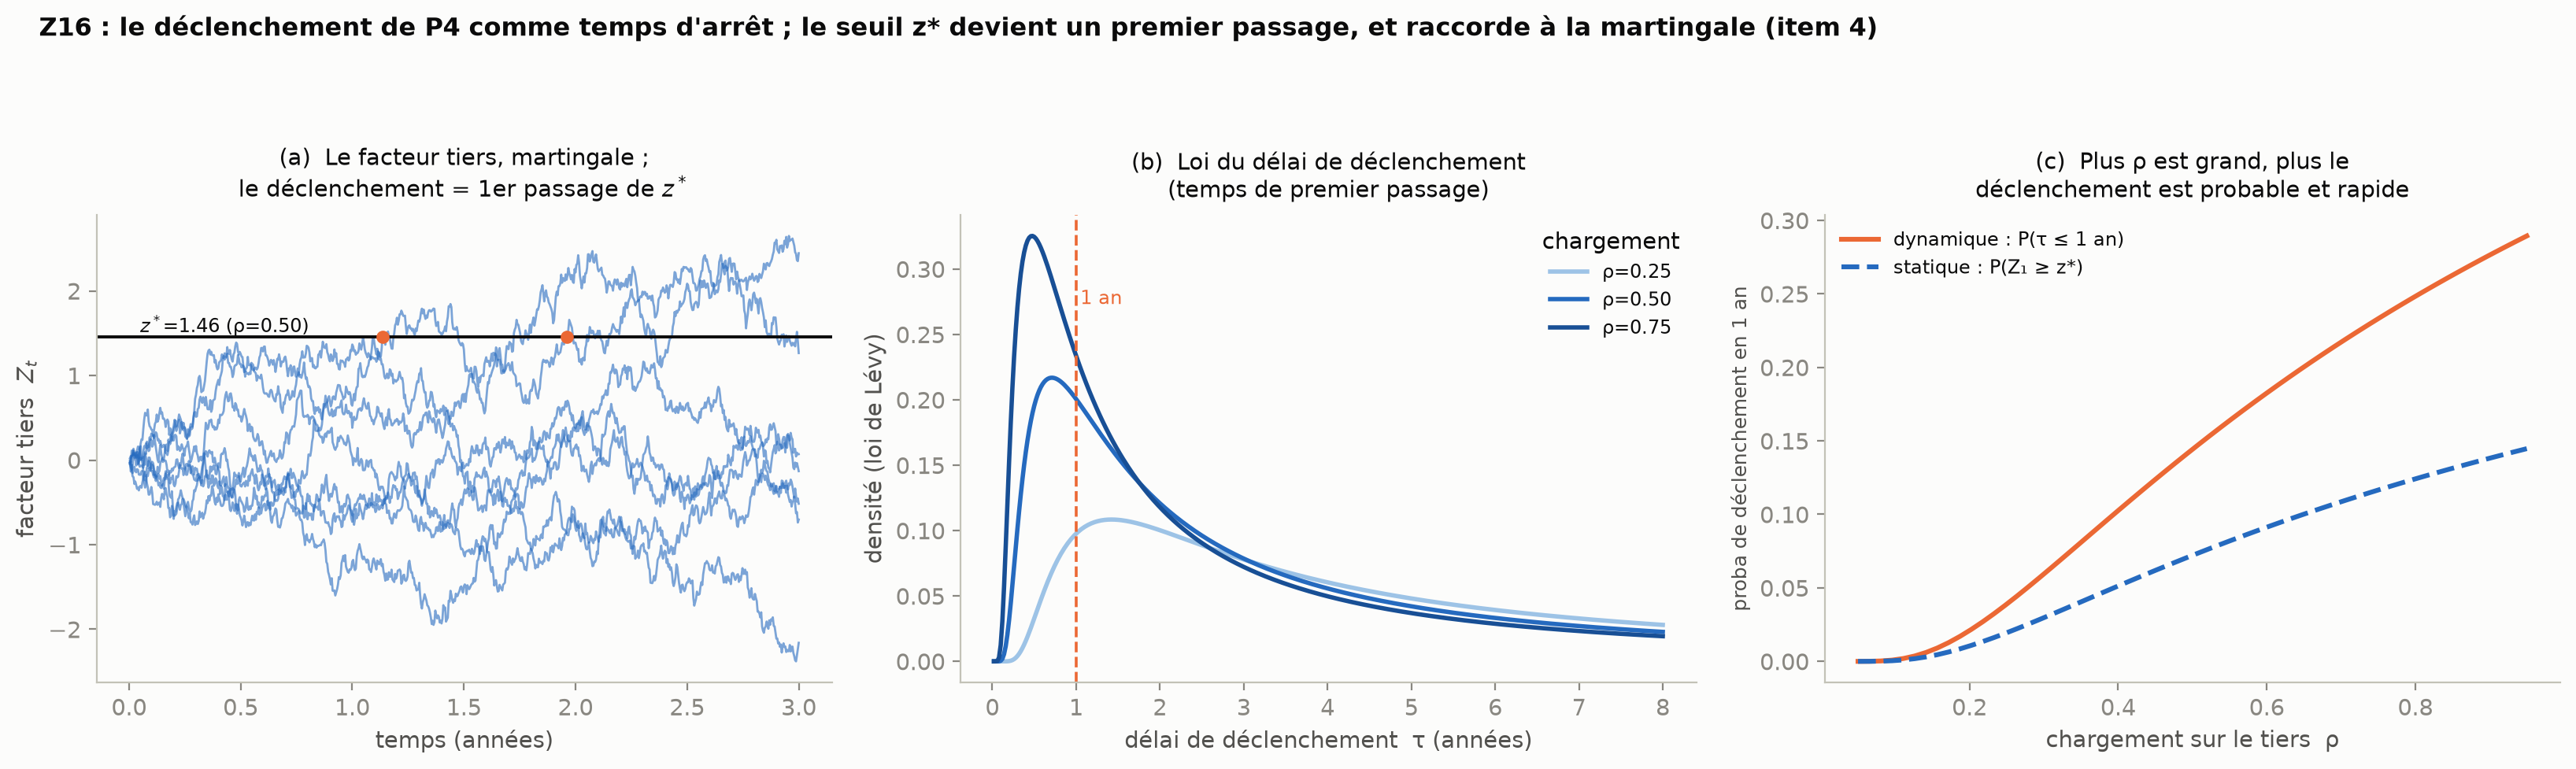
\includegraphics[width=\linewidth]{Z16_p4_temps_arret.png}
\end{column}
\begin{column}{0.43\linewidth}
\small
Si le facteur tiers est un \textbf{processus}, le seuil $z^*$ de P4 devient un \textbf{temps de
premier passage} $\tau$, un temps d'arrêt. Le \og{}moment\fg{} de déclenchement a un sens
littéral.
\medskip

Forme close (brownien, \textbf{martingale}) : $\mathbb{P}(\tau\le T)=2\Phi(-z^*/\sqrt T)$. À
$\rho=0{,}75$, $\mathbb{P}(<1\text{ an})=0{,}23$.
\end{column}
\end{columns}
\vfill
\begin{block}{}
$Z_t$ est une martingale, $\tau$ un temps d'arrêt : le seuil de P4 (piste 3) rejoint le cadre
\textbf{martingale} de l'identification (piste 4). Les pistes ne sont pas des à-côtés, c'est un
même fil.
\end{block}
\end{frame}

% =====================================================================
\begin{frame}{Points bloquants et pour la prochaine fois}
\small
\textbf{Ce qui dépend d'autres que moi}
\begin{itemize}\itemsep1pt
\item Les \textbf{deux relectures} demandées : elles lèveraient la dernière réserve sur la
      direction, et le délai de retour est le seul facteur hors de mon contrôle.
\item Le \textbf{registre d'externalisation} : le squelette d'ingestion est prêt, il n'attend
      que la donnée.
\item Le \textbf{choix de posture} sur le capital : point prédictif ou borne prudente ? À
      trancher avec Caroline, les deux sont chiffrés.
\end{itemize}
\textbf{Livré depuis le dernier point}
\begin{itemize}\itemsep1pt
\item Le chapitre sur l'\textbf{identifiabilité réécrit} : d'un verdict unique à une frontière
      en trois niveaux, et la donnée manquante devenue un chapitre à part.
\item Le mémoire \textbf{restructuré en cinq parties} selon les attendus de l'Institut (aucun
      montant de capital avant la partie Résultats), et \textbf{treize fiches} autonomes.
\end{itemize}
\vfill
\begin{block}{}
Ligne de conduite inchangée : ne jamais présenter comme mesuré ce qui est posé, ni comme
calibré ce qui n'est que corroboré.
\end{block}
\end{frame}

\end{document}
